\documentclass[9pt]{pnas-new}

\RequirePackage[english]{babel}

\templatetype{pnasresearcharticle}
\usepackage{enumitem}
\usepackage{amsmath}
\usepackage{subfigure}
\usepackage{float}

\newcommand{\set}[1]{\ensuremath{\mathbf{#1}}}
\renewcommand{\vec}[1]{\ensuremath{\mathbf{#1}}}
\newcommand{\uvec}[1]{\ensuremath{\hat{\vec{#1}}}}
\newcommand{\const}[1]{{\ensuremath{\kappa_\mathrm{#1}}}} 
\newcommand{\num}[1]{#1}

\graphicspath{{./fig/}}

\title{Reimplementing the FRIsheeping herding algorithm using fuzzy logic}

\author{Veljko Dudić}
\author{Noah Novšak}
\author{Petra Kuralt}
\author{Timotej Košir}

\affil{Collective behavior course research seminar report} 

\selectlanguage{english}

\significancestatement{A herding algorithm that uses fuzzy logic}{This study explores the integration of fuzzy logic into herding algorithms as an innovative approach to enhance adaptability and nuanced decision-making within simulated group dynamics. Initially, we build upon the Str\"{o}mbom algorithm, implemented in a Unity environment, introducing fuzzy logic to refine the behavior of entities within the herd. Afterward, our investigation extends to the implementation of herding mechanisms using genetic algorithms. This utilization of fuzzy logic and genetic algorithms aims to create a comprehensive and robust framework for simulating herding behavior in dynamic environments.}{fuzzy logic | herding algorithm  | genetic algorithm}

\equalauthors{\textsuperscript{1}N.N.(Noah Novšak), V.D. (Veljko Dudić), P.K. (Petra Kuralt), and T.K. (Timotej Košir) contributed equally to this work.}

\keywords{fuzzy logic | herding algorithm | genetic algorithm} 

\begin{abstract}
This study explores the integration of fuzzy logic into herding algorithms as an innovative approach to enhance adaptability and nuanced decision-making within simulated group dynamics. Initially, we build upon the Str\"{o}mbom algorithm, implemented in a Unity environment, introducing fuzzy logic to refine the behavior of entities within the herd. Afterward, our investigation extends to the implementation of herding mechanisms using genetic algorithms. This utilization of fuzzy logic and genetic algorithms aims to create a comprehensive and robust framework for simulating herding behavior in dynamic environments.
\end{abstract}

\dates{\textbf{\today}}
\program{BM-RI}
\vol{2023/24}
\no{CB:G}

\begin{document}

% You should only change this length when you've finalized the article contents.
\verticaladjustment{-2pt}

\maketitle
\thispagestyle{firststyle}
\ifthenelse{\boolean{shortarticle}}{\ifthenelse{\boolean{singlecolumn}}{\abscontentformatted}{\abscontent}}{}

% If your first paragraph (i.e., with the \dropcap) contains a list environment (quote, quotation, theorem, definition, enumerate, itemize...), the line after the list may have some extra indentation. If this is the case, add \parshape=0 to the end of the list environment.
\dropcap{H}erding algorithms, at their core, strive to model the behavior of a shepherd (sheepdog) endeavoring to control extensive groups of unwilling individuals (sheep).
Traditional approaches rely on predefined rules to govern the individual behavior of agents within a group, influencing their movements based on factors like proximity and alignment with neighbors~\cite{basicHerding}. While these methods capture the fundamental aspects of collective behavior, their deterministic nature might fall short in handling the inherent uncertainty and imprecision of real-world scenarios. In this context, our approach introduces another dimension to herding algorithms by incorporating fuzzy logic. This enables a more flexible and adaptive decision-making process by allowing degrees of truth between absolute true and false, thus helping the individuals in a group respond more effectively to altering environments.


As a starting point, we take the algorithm proposed by Str\"{o}mbom et al. \cite{strombom}, which has already been implemented by our predecessors in a Unity environment. Str\"{o}mbom's model employs a weighted sum of various forces to determine the sheep's movement. At the same time, the shepherd alternates between \textit{collecting} dispersed sheep and \textit{driving} the group towards a predefined goal.

In this paper, we discuss our approach to reimplementing Str\"{o}mbom's algorithm and its suggested improvements using fuzzy logic. Additionally, we explore the viability of the sheep's learning behavior through a genetic algorithm, whereby sheep incrementally improve their tactics through evolution.

\section*{Methodology}
The testing environment consists of an enclosed pasture with a barn at its edge. The $N$ agents (sheep) are randomly placed in the field with a shepherd (sheepdog), aiming to collect and drive all the sheep into the barn within a limited time. Several different algorithms can be selected to govern the behavior of each agent in the simulation.

\subsection{Str\"{o}mbom model}
Agents attempt to move away from the shepherd while staying close to their neighbors. Each agent decides on its next course of action based on the locations of itself, the shepherd $\bar{S}$, and each of its $n$ nearest neighbors $\bar{A}_{i}$. The agents are attracted to their neighbors' center of mass ($LCM$) and repelled from other agents within a boundary distance $r_a$. The shepherd repels them as well if it is closer than $r_s$.

The following components sum up all of these contributions:
\begin{enumerate}
    \item Repulsion from the shepherd:
    If the agent is within a distance $r_s$ of the shepherd, it is repelled in the opposite direction $R^s_i = A_i - S$.
    
    \item Attraction towards the local center of mass:
    The vector representing attraction is denoted at $C_i = LCM - A_i$, where $LCM = \frac{1}{n}\sum A_i$ for the agent's $n$ nearest neighbors.
    
    \item Repulsion from Other Agents:
    If there are $k$ other agents within $r_a$, the combined repulsion vector is defined as $R^a_i = \sum^k_{j=1} \frac{(A_i - A_j)}{|A_i - A_j|}$.
    
    \item Inertia and Noise:
    In each timestep, the agents maintain their previous direction $H_i$, and some random noise $\epsilon$ is added to account for unpredictability.
\end{enumerate}
Combining all these components, the movement vector in each iteration becomes $$H'_i = h H_i + c C_i + a \hat{R_i^a} + s \hat{R_i^s} + e \epsilon.$$

An entirely separate set of rules governs the shepherd's behavior. It dynamically switches between \textit{collecting} and \textit{driving}, based on the maximum distance of agents from the center of mass (either global $GCM$ or local $LCM$). If all agents are within $r_aN^\frac{2}{3}$, it attempts to position itself behind the flock to push it towards the goal. Alternatively, if any agent is farther than $r_aN^{\frac{2}{3}}$, the shepherd instead selects the most distant agent and herds it back towards the flock. The shepherd's trajectory is thus always directly toward the desired collecting or driving position. Additionally, some noise is added to the shepherd's movement as well.

% \subsection{Improvements to the model}
% The base algorithm excels when the shepherd possesses global knowledge, and the agents are attracted to the center of mass of at least half of their peers. However, its effectiveness diminishes with limited attraction among nearby agents and employing only local knowledge for the shepherd. Our goal is to enhance performance with local knowledge and reduce the dependence on agent behavior. We propose two essential modifications: avoiding already collected groups and implementing a modified heuristic for selecting the target agent in collection mode.
% \begin{enumerate}
%     \item \textbf{Avoidance of already collected groups (previous algorithm with angle calculation):}
%     A modification is introduced to avoid breaking up already collected groups of agents during the herding process. Instead of taking a straight path towards the furthest agent from the center of mass (GCM/LCM), the shepherd follows an arc around the calculated GCM/LCM. This approach ensures a constant distance from the GCM/LCM, preventing unintended group disruptions. However, this adjustment may extend the time it takes for the shepherd to reach the desired collecting position, particularly in scenarios where the shepherd is considerably distant from the GCM/LCM compared to the collecting position.
%     \item \textbf{Avoidance of already collected groups and obstacles (new version - weighted sum):}
%     When collecting agents, the shepherd avoids disrupting already gathered groups by circling the herd in an arc. The desired heading is a weighted combination of a direct target vector $(H^d)$ and an arc movement vector $(H^a)$. The arc movement is calculated as $$H^a = \sum^n_{i=1}\frac{1}{(|A_i - S|)^2} \cdot H_{i^\bot},$$ where S is the shepherd's position, $A_1,\dots, A_n$ are the positions of known agents, and $H^i$ is a vector perpendicular to $\mathop{A{}}\limits^\wedge -\mathop{S{}}\limits^\wedge$ based on the target position relative to the center of mass.
    
% The shepherd's desired heading ($\hat{H_s}$) is computed as: $$\rho_d\hat{H{_d}} + \rho_\alpha\hat{H{_\alpha}} + \rho_o\hat{H_o},$$ with weights $\rho_d$ and $\rho_\alpha$ determined by the distance ($d$) to the nearest agent:

% $$\rho_d = 1, if \hspace{0,3cm} d \geq r_r, else \hspace{0,3cm}  \frac{d}{(r_r)},$$
% $$\rho_\alpha = 0, if \hspace{0,3cm} d \geq r_r, else \hspace{0,3cm} \frac{r_r - d}{r_r}.$$
% When distant from agents, the shepherd moves straight towards the target, transitioning to an arc movement within $r_r$ distance of an agent. The $r_r$ parameter is equal to the $r_s$ parameter of agents, assuming the shepherd adjusts its path upon approaching that distance.

% For field navigation, repulsion from obstacles ($R^o_s$) is added, calculated as: $$R^o_s =  \sum^j_{i=1}{\frac{1}{|S - O_i|}(S - O_i)},$$ where $O_1, ..., Oi$ are obstacle boundary points within $r_o$ distance. A small constant $\ rho_o$ weights this vector.
% \end{enumerate}

\subsection{Fuzzy logic}
We defined the existing \textit{crisp} model in the previous section. Now, we will try to describe its \textit{fuzzy} counterpart. Using fuzzy logic may introduce a more nuanced and realistic decision-making process for determining the behavior of each agent.

As a starting point, we will take the model proposed by "Boids with a fuzzy way of thinking"~\cite{bajec2003boids}. They find the most important aspect of flocking behavior is the alignment function. Then, we will add an additional component to model the shepherd guiding the flock.
The described model uses three linguistic variables: the relative heading difference $H$ coded by the values $LEFT$, $RIGHT$, and $SAME$~\ref{membership}, the relative speed difference $S$ coded by $SLOWER$, $FASTER$, and $SAME$~\ref{membership}, and the significance $SIG$ of each neighboring agent, coded by $HIGH$ and $LOW$~\ref{membership}.
Using these linguistic variables, the alignment steering function is represented by the following rules:
\begin{verbatim}
if (SIG is LOW) or (H is SAME) then H' is SAME,
if (SIG is HIGH) and (H is LEFT) then H' is LEFT,
if (SIG is HIGH) and (H is RIGHT) then H' is RIGHT,
if (SIG is LOW) or (S is SAME) then S' is SAME,
if (SIG is HIGH) and (S is SLOWER) then S' is SLOWER,
if (SIG is HIGH) and (S is FASTER) then S' is FASTER,
\end{verbatim}
Our proposal for adding a shepherd is to model it with more or less the same alignment rules but using different weights and membership functions.

\begin{figure}[ht]\centering
    \subfigure[Heading]{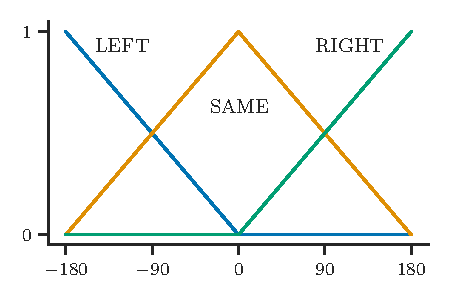
\includegraphics[width=0.3\textwidth]{fig/heading_membership}}
    \subfigure[Speed]{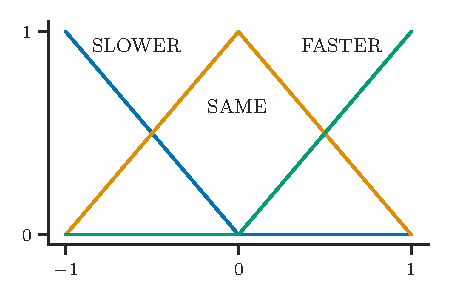
\includegraphics[width=0.3\textwidth]{fig/speed_membership}}
    \subfigure[Significance]{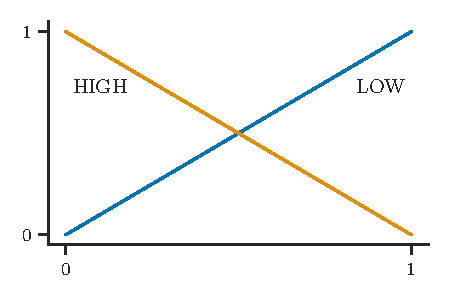
\includegraphics[width=0.3\textwidth]{fig/significance_membership}}
    \caption{Membership functions}
    \label{membership}
\end{figure}

The first step in implementing this model is to fuzzify the inputs, i.e., taking the agents' positions and current headings to determine the degree to which they belong to each of the appropriate fuzzy sets via the aforementioned membership functions.
The next step is to combine the fuzzy inputs according to the proposed rules into a single number, the antecedent. Then, create a new fuzzy set, the consequent, and reshape it using the antecedent.
Then, finally, all of the rule outputs are aggregated into a single fuzzy set and defuzzified into a single numeric output.

\subsection{OCEAN model}
To further extend the fuzzy logic model, we use the OCEAN personality model, generally used to describe people, to individualize the agents~\cite{fuzzylogic}. 

As defined in social science and psychology, our personalities shape our thoughts, feelings, and behaviors, distinguishing us from other individuals. Modeling heterogeneous sheep requires considering personalities, as individuals with diverse traits react differently to the same situation. The Five-Factor personality model, known as OCEAN, categorizes personalities into five contributing factors:
\begin{enumerate}
  \item \textbf{Openness (O)} reflects the degree of curiosity and creativity, indicating preferences for novelty and variety.
  \item \textbf{Conscientiousness (C)} describes the level of organization and care exhibited in collective activities
  \item \textbf{Extraversion (E)} related to the degree of energy, sociability, and outgoingness.
  \item \textbf{Agreeableness (A)} represents a tendency to exhibit compassion and cooperation rather than suspicion and antagonism towards others.
  \item \textbf{Neuroticism (N)} indicates the tendency to experience unpleasant emotions easily, such as anger, anxiety, depression, or vulnerability, and is the opposite of emotional stability.
\end{enumerate}
Agents are modeled with these traits to achieve more realistic crowd behavior.

\subsection*{Fuzzy Inference Model}
The first implementation is based on~\cite{bajec2003boids} and does not use an intermediate pathing algorithm. Each sheep has its own personality, and using the position and speed of sheep in a local environment, we use our fuzzy inference system to return a new heading and speed for all sheep. These values are directly used for the movement of the given sheep.\\
The second implementation is based on~\cite{fuzzylogic} and builds on top of the Str\"{o}mbom algorithm. Instead of directly obtaining the speed and angle of the sheep, we derive new parameters for Str\"{o}mbom from the personality of each individual agent and assign the parameters from defined fuzzy rules, such as:
\begin{verbatim}    
if (Extraversion is POS) and (Agreeableness is POS) then k neighbors HIGH
if (Neuroticism is POS) then added noise is HIGH
\end{verbatim}
Each sheep's personality is based on the OCEAN model but excludes the conscientiousness aspect. The inputs of the fuzzy inference system are, in this case, the personality of a sheep and the previous Str\"{o}mbom parameters, and the outputs are the new parameters.  


\subsection{Genetic algorithm}
The second focus of the article is making sheep dynamics less scripted but learned. We plan to achieve this by representing the sheep as autonomous agents that utilize a genetic algorithm (GA) to evolve their herding strategies incrementally. 

GAs are optimization algorithms inspired by the concept of natural selection. The process starts by generating an initial population of potential solutions. Each solution is assessed using a cost function, and solutions with higher fitness are more likely to be selected for reproduction. The chosen individuals undergo crossover and mutation, eventually replacing the less fit individuals in the population. This cycle repeats for multiple generations, refining the solutions over time.

Regarding collective behavior, we need to modify the traditional GA by adding some changes presented in Thomas Miconi's "A Collective Genetic Algorithm"\cite{miconi2001collective}. Since we can not evaluate a single agent but rather the population as a whole, we randomly select two sheep and separately remove them to evaluate their impact on the whole herd. We then create offspring through crossover and mutation. The less valuable sheep, as determined by their effect on the collective herding fitness, are then replaced by the offspring. The sheep's genotype will be represented as a vector so that we can use it as our sheep's decision model. Currently, the plan is to use a simple three-layer artificial neural network. The input layer will consist of an input vector containing information about distances to other sheep and shepherds, and the output layer will return the angular direction and speed of the sheep's movement. 

The initial suggestion for the cost function is a weighted sum between the time it took for all the sheep to enter the barn and the distances separating them in a herd. The optimization strategy is designed to encourage sheep to form a cohesive pack while simultaneously maximizing their evasiveness. Examples of similar implementations using ANN models can also be observed in simulating the collective behavior of zebrafish~\cite{7496361} and robots~\cite{cazenille2018modelling}, albeit using supervised training of the neural network agent's models instead of genetic algorithms. 

\section*{Results}
We have extended the FRIsheeping Unity project to include the proposed Fuzzy Logic models, moving away from planned pathing algorithms to mimic the erratic behavior of the sheep herd. The improvement allows for more dynamic and unpredictable collective movements, as each sheep now exhibits individualized responses influenced by unique personality traits.

\begin{figure}[H]
    \centering
    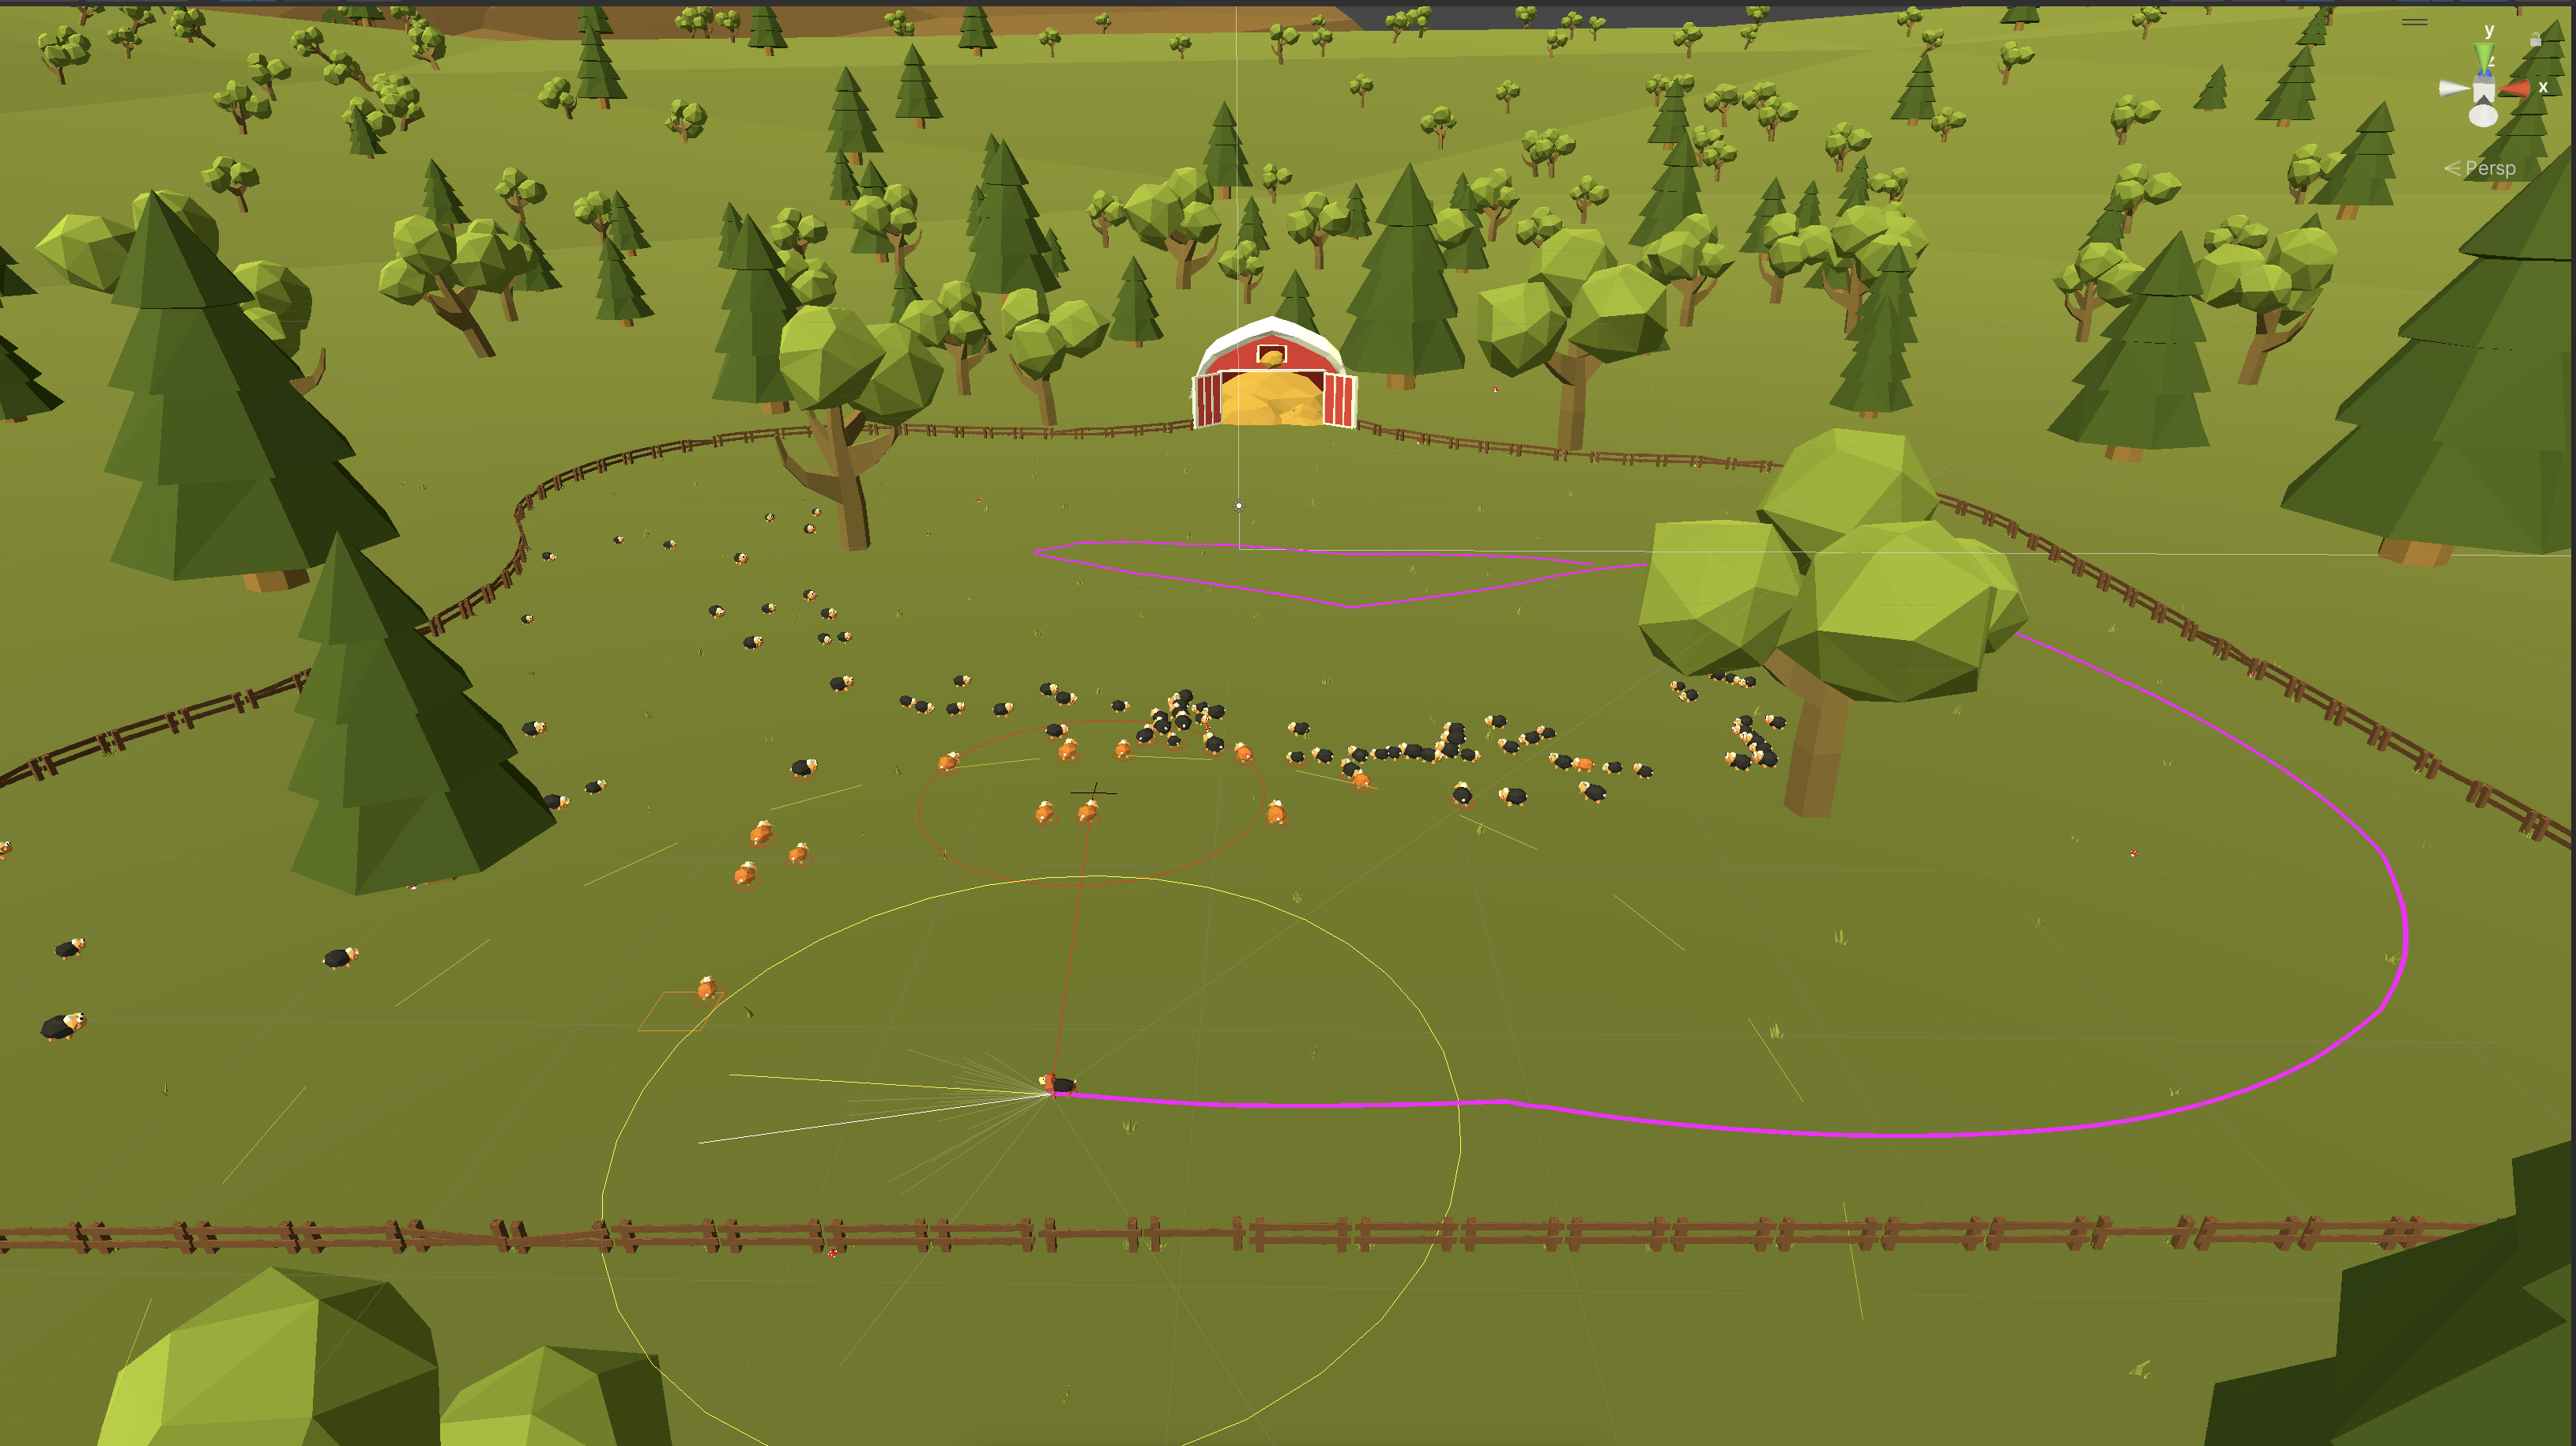
\includegraphics[width=\columnwidth]{fig/strombom2.png}
    \caption{An example of our setup in Unity environment}
\end{figure}


\section*{Discussion}
The two proposed fuzzy logic inference models give us insight into different fuzzy logic applications for simulating herding dynamics. The first approach, stemming from~\cite{bajec2003boids}, embraces simplicity by directly incorporating fuzzy logic into the movement of each sheep. The personalized nature of sheep behavior, dictated by OCEAN personality, allows for a decentralized decision-making process. In contrast, the second implementation, inspired by~\cite{fuzzylogic} and building upon the Str\"{o}mbom algorithm, introduces a layer of complexity by deriving new parameters based on individual personality traits. In both approaches, a fuzzy inference system determines the relationships between personality traits and decision preferences.


% A variety of simulations and validation experiments are implemented in our developed application. The experimental results show that the proposed model can ...

% In the future, we intend to ...

% \acknow{distribution of labor}
\showacknow % Display the acknowledgments section

% If you see unexpected formatting errors, try commenting out this line
% as it can run into problems with floats and footnotes on the final page.
% \pnasbreak % Splits and balances the columns before the references.

\begin{multicols}{2}
\section*{\bibname}
% Bibliography
\bibliography{./bib/bibliography}
\end{multicols}

\end{document}